%% LaTeX Beamer presentation template (requires beamer package)
%% see http://bitbucket.org/rivanvx/beamer/wiki/Home
%% idea contributed by H. Turgut Uyar
%% template based on a template by Till Tantau
%% this template is still evolving - it might differ in future releases!

\documentclass{beamer}

\mode<presentation>
{
\usetheme{Warsaw}

\setbeamercovered{transparent}
}

\usepackage[polish]{babel}
\usepackage[utf8]{inputenc}

% font definitions, try \usepackage{ae} instead of the following
% three lines if you don't like this look
\usepackage{mathptmx}
\usepackage[scaled=.90]{helvet}
\usepackage{courier}
\usepackage{graphicx}


\usepackage[T1]{fontenc}


\title{Peer-to-peer web objects cache}

%s\subtitle{Chaum, Crepeau, Damgard}

% - Use the \inst{?} command only if the authors have different
%   affiliation.
%\author{F.~Author\inst{1} \and S.~Another\inst{2}}
\author{Tomasz Drwięga}

% - Use the \inst command only if there are several affiliations.
% - Keep it simple, no one is interested in your street address.
% \institute[Universities of]
% {
% \inst{1}%
% Department of Computer Science\\
% Univ of S
% \and
% \inst{2}%
% Department of Theoretical Philosophy\\
% Univ of E}

\date{20.03.2013 / Seminary}


% This is only inserted into the PDF information catalog. Can be left
% out.
\subject{Talks}



% If you have a file called "university-logo-filename.xxx", where xxx
% is a graphic format that can be processed by latex or pdflatex,
% resp., then you can add a logo as follows:

% \pgfdeclareimage[height=0.5cm]{university-logo}{university-logo-filename}
% \logo{\pgfuseimage{university-logo}}


% If you wish to uncover everything in a step-wise fashion, uncomment
% the following command:

%\beamerdefaultoverlayspecification{<+->}

\begin{document}

\begin{frame}
\titlepage
\end{frame}

\begin{frame}
\frametitle{Outline}
\tableofcontents
% You might wish to add the option [pausesections]
\end{frame}


\section{Problem statement}

\begin{frame}
\frametitle{Problem Statement}

\begin{block}{Content provider}
A lot of requests can cause server to become ``flooded'' (``swamped'')
\end{block}
\pause
\begin{block}{Network admins}
A lot of outgoing traffic for the same resources results in lower QoS.
\end{block}
\pause
\begin{block}{Users}
Requesting large files from remote servers can cause significant delays.
\end{block}
\end{frame}


\section{Previous work}
\subsection{Harvest (Squid) object cache}

\begin{frame}
\frametitle{Squid object cache}

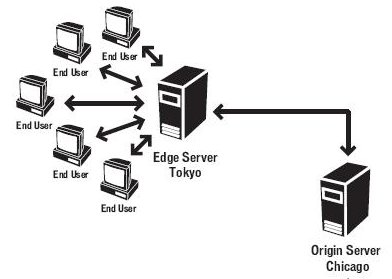
\includegraphics[width=0.8\linewidth]{media_server2_edge.jpg}

\begin{block}{}
A simple solution: introduce servers that will replicate original content.
\end{block}

\end{frame}


\begin{frame}
\frametitle{Hierarchical cache}
\begin{block}{}
Multiple cache servers can be organized into hierarchy \cite{chankhunthod1995hierarchical}.
\end{block}
\begin{center}
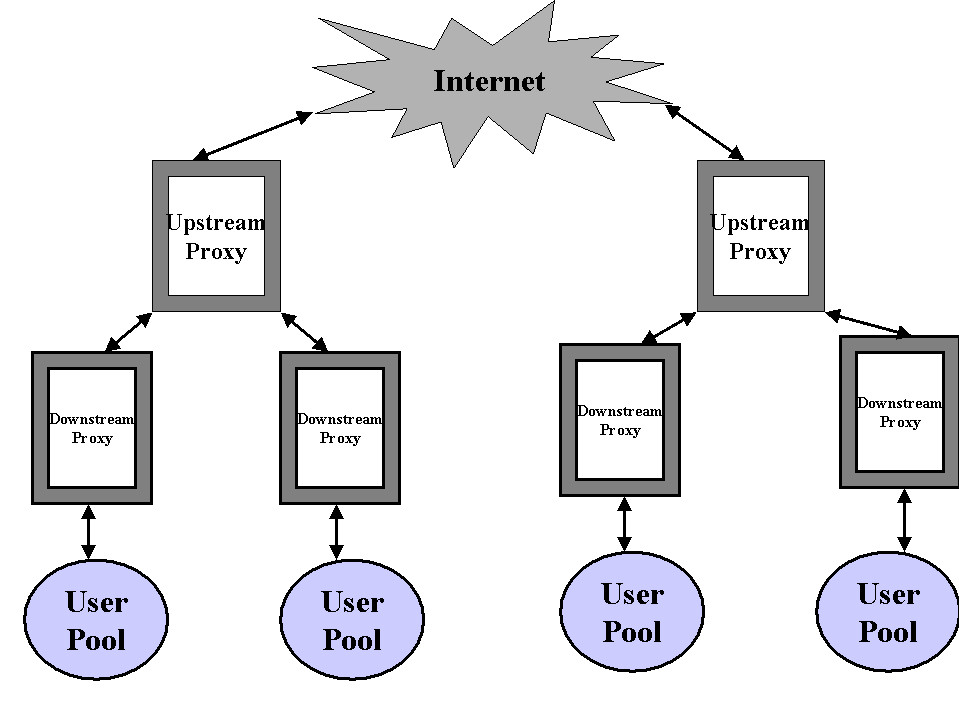
\includegraphics[width=0.54\linewidth]{fig5.jpg}
\pause
\begin{block}{}
Leaf servers can transfer resources among themselves (cooperative caching). 
However it leads to excessive communication \cite{povey1997distributed} \cite{wolman1999scale}.
\end{block}
\end{center}

\end{frame}

\subsection{Consistent Hashing}

\begin{frame}
\frametitle{Towards Consistent Hashing \cite{karger1997consistent}}
\begin{block}{}
The main problem with multiple caching servers was to determine which server
might contain the resource. 
\end{block}

\pause
\begin{block}{Naive Distribution}
Let's assume we are searching for resource $R$ in server $S$: 
\begin{equation*}
S \equiv hash(R) \bmod n
\end{equation*}
\end{block}

\pause
\begin{block}{Serious Flaw of Naive Distribution}
When new servers are added or removed the whole content has to be remapped to new targets.
\end{block}

\end{frame}


\begin{frame}
\frametitle{Consistent hashing}

\begin{block}{}
We would like to optimize the process of adding/removing nodes so that new nodes
takes their fair share of objects from others.
\end{block}

\begin{columns}[c]
\column{0.58\textwidth}

\begin{center}
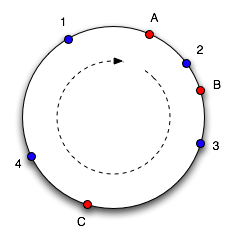
\includegraphics[width=0.75\linewidth]{consistent_hashing_1.png}
\end{center}

\column{0.38\textwidth}
\begin{block}{Consistent hashing}
Each node (as well as each resource) is mapped to a point on unit circle.
Node is responsible for keys after its point and its successor's \cite{karger1999web}. 
\end{block}

\end{columns}

\end{frame}



\subsection{DHT - Kademlia}

\begin{frame}
\frametitle{Distributed Hash Table}

\begin{block}{Distributed Hash Table}
Decentralized (autonomous), self-organized peer-to-peer system that provides service similar to a hash table.
DHTs should also be fault tolerant and scalable.
\end{block}

\pause
\begin{block}{}
DHTs research was originally motivated by existing systems:
\begin{description}
  \item[Napster] P2P with a central index handling searches
  \item[Gnutella] P2P with flooding query model
  \item[Freenet] distributed, but no guarantee that data will be found
\end{description}
\end{block}

\begin{block}{Four main DHTs (2001)}
CAN, Chord, Pastry, Tapestry
\end{block}

\end{frame}

\begin{frame}
\frametitle{Kademlia \cite{maymounkov2002kademlia} (2002)}
\begin{block}{}
Like other DHTs, Kademlia contacts only $O(\log n)$ nodes.
\end{block}

\pause

\begin{block}{}
Each node has a 160 bit key. A node has a routing table that stores
lists ($k$-buckets) of nodes whose keys share a prefix of length $i$ with its key,
but differ from it on bit $i+1$. Those $k$-buckets exists for each $i \in [0, 160)$
\end{block}

\begin{center}
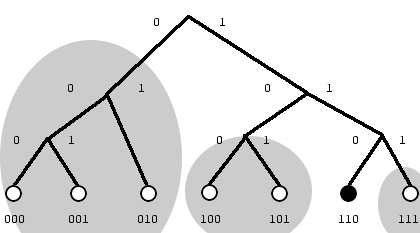
\includegraphics[width=0.55\linewidth]{kademlia.png}
\end{center}

\end{frame}

\begin{frame}
\frametitle{Kademlia - XOR metric}

\begin{block}{}
Kademlia uses XOR metric to define distance, which means that keys with long common prefix are close. It simplifies formal analysis,
correctness proof and implementation.
\end{block}

\pause

\begin{block}{}
Protocol messages:
\begin{description}
\item[PING] verifies that a node is still connected,
\item[STORE] asks a node to store (key, value) pair
\item[FIND\_NODE] given node ID returns $k$ closest nodes
\item[FIND\_VALUE] given object ID returns $k$ closest nodes or corresponding value
\end{description}
\end{block}

\end{frame}

\begin{frame}
\frametitle{Kademlia routing comparison}

\begin{block}{}
XOR metric simplifies routing algorithm - unlike Pastry or Tapestry same algorithm is used during the whole process.
\end{block}

\pause

\begin{block}{}
Because XOR is unidirectional (for any $x$ and $\Delta$ there is only one $y$ such that $d(x, y) = \Delta$) lookups for
the same key converge along the same path. 

So it is possible (like in design of Tapestry) to cache (key, value) pairs along the path. 
\end{block}

\pause

\begin{block}{}
This caching speeds-up retrieving popular content from the network
\end{block}

\end{frame}

\section{P2P Caching}
\begin{frame}
\frametitle{P2P Caching}

\begin{block}{}
Instead of downloading resource from original server we perform lookup
in Kademlia DHT.
\end{block}

\begin{block}{Potential benefits}
\begin{itemize}
  \item Large resources can be obtained faster (nodes are in the same LAN)
  \item WAN network bandwidth is saved
\end{itemize}
\end{block}

\end{frame}

\begin{frame}
\frametitle{P2P Caching - Implementation}

\begin{block}{First attempt: Javascript browser plugin}
An easy-to-install plugin that uses HTML5 APIs.

\textbf{Why not?} Requests have to be processed synchronously. 
\end{block}

\pause
\begin{block}{Native Client plugin for Chrome}
Easy-to-install, good performance, but limited only to Chrome.

\textbf{Why not?} Lack of documentation, unsufficient APIs.
\end{block}

\pause
\begin{block}{Fallback: Proxy \cite{guha2002improving}}
Proxy server written in Python using Twisted framework and Entangled library implementing Kademlia.

\textbf{Drawback:} Requires additional configuration
\end{block}

\end{frame}

\section{Challenges}
\begin{frame}
\frametitle{Challenges}

\begin{block}{Caching logic}
\begin{itemize}
  \item To cache or not to cache? That is the question!
  \item Removal of old items 
\end{itemize}
\end{block}

\pause
\begin{block}{Requests balancing}
Requests for items from the same source can be routed to completely different 
parts of network (random hashing keys).
\end{block}

\pause
\begin{block}{Caching and Streaming of partial content}
\begin{itemize}
  \item Cache parts of content
  \item Stream data instead of sending whole files at once
\end{itemize}
\end{block}

\end{frame}

\subsection{Caching logic}
\begin{frame}
\frametitle{Caching logic \cite{motwani1995randomized} - multilevel cache}
\begin{columns}[c]

\column{0.4\textwidth}
\begin{center}
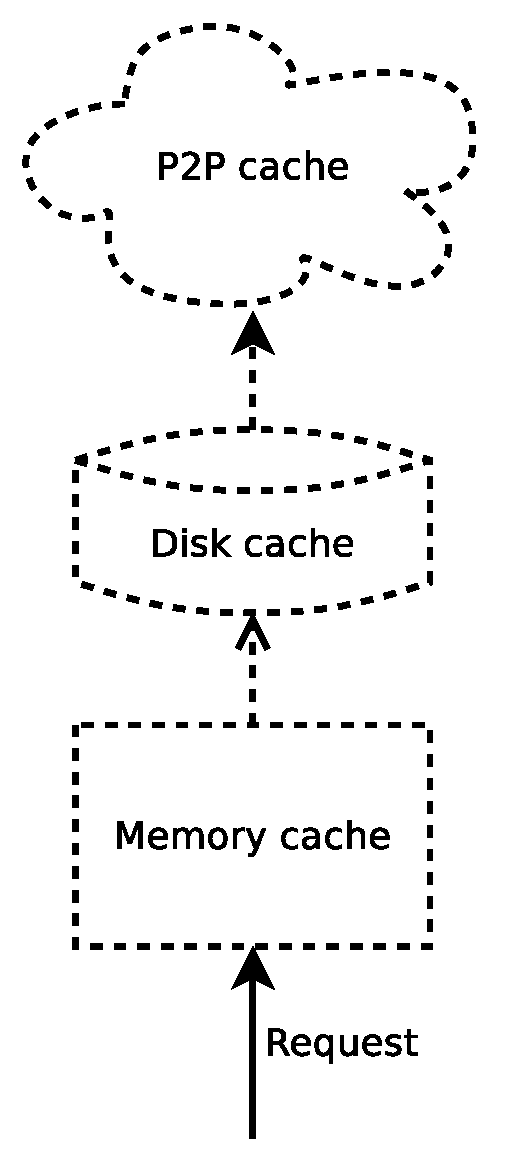
\includegraphics[width=0.65\linewidth]{cache1.eps}
\end{center}

\column{0.4\textwidth}
\begin{block}{}
Retrieving an item from disk or P2P cache increases latency.
\end{block}
\begin{block}{}
We don't know if the item even exists in P2P cache.
\end{block}

\end{columns}
\end{frame}

\subsection{Requests balancing}
\begin{frame}
\frametitle{Requests balancing}

\begin{block}{}
We could use skip graphs \cite{aspnes2007skip} to ask for keys in some range 
(for instance resources from same domain). 
\end{block}

\begin{block}{}
Multiple files from same domain could be also stored as one resource
in P2P network - we could retrieve whole bunch when any resource is requested
(keywords based searching).
\end{block}

\end{frame}

\subsection{Caching/Streaming partial content}

\begin{frame}
\frametitle{Streaming partial content}
\begin{block}{}
Increasing demand on multimedia content (e.g. Youtube)
\end{block}

\begin{block}{}
Should parts of a file be stored separately?
\end{block}

\begin{block}{}
We need to retrieve parts in order to allow streaming of content.
\end{block}

\end{frame}

\begin{frame}[allowframebreaks]
\frametitle{References}
\bibliographystyle{abbrv}
\bibliography{document.bib}
\end{frame}


\end{document}
